\documentclass[10pt,dvips,twoside,reqno]{amsart}
\usepackage{epsfig}
\usepackage[authoryear]{natbib}
\setlength{\oddsidemargin}{0in}
\setlength{\evensidemargin}{0in}
\setlength{\topmargin}{-0.25in}
\setlength{\headheight}{0.1in}
\setlength{\headsep}{0.15in}
\setlength{\topskip}{0in}
\setlength{\footskip}{0.15in}
\setlength{\textwidth}{6.5in}
\setlength{\textheight}{9in}

%differential operators
\newcommand{\grad}{\nabla}
\newcommand{\deld}{\nabla \cdot}
\newcommand{\lap}{\Delta}
%boldface in math mode
\newcommand{\bm}[1]{\mbox{{\boldmath ${#1}$}}}
% vectors and tensors
\renewcommand{\vec}[1]{{\bf #1}}
\newcommand{\gvec}[1]{\mbox{{\boldmath ${#1}$}}}
\newcommand{\ten}[1]{\bar{\bm{#1}}}
%derivatives
\newcommand{\od}[2]{\frac{d {#1}}{d {#2}}}
\newcommand{\ods}[2]{\frac{d^2{#1}}{d {{#2}^2}}}
\newcommand{\pd}[2]{\frac{\partial {#1}}{\partial {#2}}}
\newcommand{\pds}[2]{\frac{\partial^2{#1}}{\partial {{#2}^2}}}
\newcommand{\pdsm}[3]{\frac{\partial^2{#1}}{\partial {#2}\,\partial {#3}}}
%funtional analysis
\newcommand{\abs}[1]{\left| #1 \right|}
\newcommand{\norm}[1]{\left\| #1 \right\|}
\newcommand{\iprod}[2]{\left( #1, #2 \right)}
\newcommand{\dprod}[2]{\left\langle #1, #2 \right\rangle}
%real numbers
\newcommand{\field}[1]{\mathbb{#1}}
\newcommand{\R}{\field{R}}
%funciton spaces
\newcommand{\M}{\mathcal{M}}
%delimiters
\newcommand{\pl}{\left(}
\newcommand{\pr}{\right)}
\newcommand{\sbl}{\left[}
\newcommand{\sbr}{\right]}
\newcommand{\dbl}{\left[\hspace{-0.05cm}\left[}
\newcommand{\dbr}{\right]\hspace{-0.05cm}\right]}
\newcommand{\cbl}{\left\{ }
\newcommand{\cbr}{\right\} }
\newcommand{\eqn}[1]{equation \ref {eq:#1}} 
\newcommand{\Eqn}[1]{Equation \ref {eq:#1}} 
\newcommand{\eqnst}[2]{equations \ref{eq:#1} and \ref{eq:#2}} 
\newcommand{\Eqnst}[2]{Equations \ref{eq:#1} and \ref{eq:#2}} 
\newcommand{\eqns}[2]{equations \ref{eq:#1}--\ref{eq:#2}} 
\newcommand{\Eqns}[2]{Equations \ref{eq:#1}--\ref{eq:#2}}
\newcommand{\msection}[1]{ \vspace{.2in} {\noindent \bf #1}.}
\renewcommand{\for}{\mbox{for}\quad}
%\newcommand{\for}{\mbox{for}\quad}
\newcommand{\argmin}{\mbox{argmin}}
\newcommand{\argmax}{\mbox{argmax}}
\newcommand{\fig}[1]{figure \ref{fig:#1}} 
\newcommand{\Fig}[1]{Figure \ref{fig:#1}} 
\newcommand{\figst}[2]{figures \ref {fig:#1} and \ref {fig:#2}} 
\newcommand{\Figst}[2]{Figures \ref {fig:#1} and \ref {fig:#2}} 
\newcommand{\figs}[2]{figures \ref{fig:#1}--\ref{fig:#2}} 
\newcommand{\Figs}[2]{Figures \ref{fig:#1}--\ref{fig:#2}}
\newcommand{\tab}[1]{table \ref {tab:#1}} 
\newcommand{\Tab}[1]{Table \ref {tab:#1}} 
\newcommand{\tabst}[2]{tables \ref {tab:#1} and \ref {tab:#2}} 
\newcommand{\Tabst}[2]{Tables \ref {tab:#1} and \ref {tab:#2}} 
\newcommand{\tabs}[2]{tables \ref{tab:#1}--\ref{tab:#2}} 
\newcommand{\Tabs}[2]{Tables \ref{tab:#1}--\ref{tab:#2}}
\newtheorem{theorem}{Theorem}
\newenvironment{neqnarray}[1]{\begin{minipage}[t]{6.5in}  \begin{minipage}[b]{1.0in} #1 \end{minipage}  \begin{minipage}[b]{5.5in}\begin{eqnarray}}{\end{eqnarray}\end{minipage}\end{minipage}}
\newcommand{\bneqnarray}[2]{\\ \\ \fbox{\begin{neqnarray}{#1} #2 \end{neqnarray}}\\ \\ \noindent} 
\begin{document}

\begin{center}
{\bf Notes on Degenerate Parabolic Equations Modeling Flow and Transport in Porous Media \\}
Chris Kees\\
Center for Research in Scientific Computation, Department of Mathematics, North Carolina State University, Raleigh, NC 27695-8205, email: {\texttt chris\_kees@ncsu.edu} \\
April 5, 2004
\end{center}

We're interested in the following degenerate advection-diffusion
equations with various initial and boundary conditions. We will only
consider $1D$ models for now and focus on the behavior of the
solutions near the degeneracy.

\msection{Solute Transport with Adsorption} Solute transport in saturated porous media under the assumption of local equilibrium mass transfer with the solid phase can be modeled as
\begin{equation}
  \label{eq:react}
  (C + \frac{\rho_b}{\omega} K C^r)_t + F_0 C_x - D_0 C_{xx}  = 0 
\end{equation}
where $C$ is the aqueous phase concentration, $0<r<1$ and $K$ are the
Freundlich isotherm parameters, $\rho_b$ is the bulk density of the
solid phase, $\omega$ is the porosity, $D_0$ is the hydrodynamic
dispersion coefficient, and $F_0$ is the mean pore velocity (c.f.
\citep{Kanney_02}). Since we're interested in the behavior near
$C=0$ we assume $\frac{\rho_b}{\omega} K=1$ and apply a change of
variables, $C=u^{1/r}$. We will consider the leading order behavior
near $C=0$ thus we use the asymptotic approximation $u^{1/r} + u \sim
u$ since $1/r > 1$ ($f \sim \phi$ means $f = \phi + o(\phi)$). The
resulting simplified model is
\begin{equation}
  \label{eq:reactTrans}
  u_t + F_0(u^{1/r})_x - D_0 (u^{1/r})_{xx} = 0
\end{equation}
This problem is degenerat in two ways. First, neglecting diffusion we
have that the characteristic speeds are $F_0 u^{1/r -1}/r = 0$ at
$u=0$. Second, we likewise that the diffusion coefficient is $D_0
u^{1/r -1}/r =0$ at $u=0$.

\msection{Two-Phase Flow Equation} In one space
dimension, the standard model for incompressible twophase flow in a homogeneous
porous medium reduces to an equation for the wetting phase saturation
$S$:
\begin{equation}
  \label{eq:buckleyLeverett}
  S_t + F(S)_x  - [D(S) S_x]_x  = 0 
\end{equation}
where
\begin{eqnarray}
  \label{eq:buckleyLeverettCoeff}
  D &=& -\frac{k_i}{\omega \mu_w} \frac{k_{rw} k_{rn}}{\frac{\mu_n}{\mu_w} k_{rw} + k_{rn}}  \od{p_c}{S}\\
F &=& \frac{k_i \mu_n}{\omega \mu_w} \frac{k_{rw}}{\frac{\mu_n}{\mu_w} k_{rw} + k_{rn}} q_t +\frac{k_i}{\omega \mu_w} \frac{k_{rw} k_{rn}}{\frac{\mu_n}{\mu_w} k_{rw} + k_{rn}}(\rho_w - \rho_n) g_x 
\end{eqnarray}
The constants in the equation are $k_i$ (permeability), $\omega$
(porosity), $\mu_w$ (wetting phase viscosity), $\mu_n$ (non-wetting
phase viscosity), $\rho_w$ (wetting phase density), $\rho_n$
(non-wetting phase density), $q_t$ (total velocity), and $g_x$
(gravitational acceleration). The nonlinear constitutive relations are the relative permeabilities, $k_{rw}$ and $k_{rn}$, and the capillary pressure $p_c$, which we will specify after considering a related model. 

\msection{Richards' Equation for Air/Water Systems} Starting from the two-phase flow equation, if we assume $\rho_w >> \rho_n$ and $\mu_n << \mu_w$ we obtain
\begin{eqnarray}
F &\approx& \frac{k_i k_{rw}}{\omega \mu_w} \rho_w  g_x \\
D &\approx& -\frac{k_i k_{rw}}{\omega \mu_w} \od{p_c}{S} 
\end{eqnarray}
The resulting equation is identical to Richards' equation for variably saturated flow.

\msection{Van Genuchten-Mualem Closure Relations} Using Van Genuchten's capillary pressure model and Mualem's permeability
model we can write the nonlinearities for two-phase flow and Richards' equation as 
\begin{eqnarray}
\od{p_c}{S} &=& \frac{m-1}{m \alpha}\pl S^{-1/m} - 1 \pr^{-m}(S^{-1/m - 1}) \\
k_{rw} &=& S^{1/2} \sbl 1-(1-S^{1/m})^m \sbr^2 \\
k_{rn} &=& (1-S)^{1/2}(1-S^{1/m})^{2m}
\end{eqnarray}
where $0<m<1$ and $\alpha>0$ are constants.  

\msection{Degenerate Coefficients} We will focus on the behavior of
the coefficients at $S=1$. For simplicity we will set $v_t=0$, $\alpha
= \omega = k_i = \rho_w = \mu_w = \mu_n = 1$, $g_x = \pm 1$, and
$\rho_n = 0$.  The case $v_t=0$ is sometimes called gravity
segregation or counter-current flow since there is no net movement of
the fluid mixture and buoyancy is the only driving force.  The
nonlinear coefficients are plotted in figures \ref{blCoeff} and
\ref{reCoeff}. Note that the coefficients are degenerate in several
different ways. First, as with the reactive transport model above, we
can have that the characteristic seeds and diffusion are zero. Second,
we can have loss of Lipschitz continuity at $S=1$.  Finally, we can
also have $D \rightarrow \infty$ as $S \rightarrow 1$.
\begin{figure}
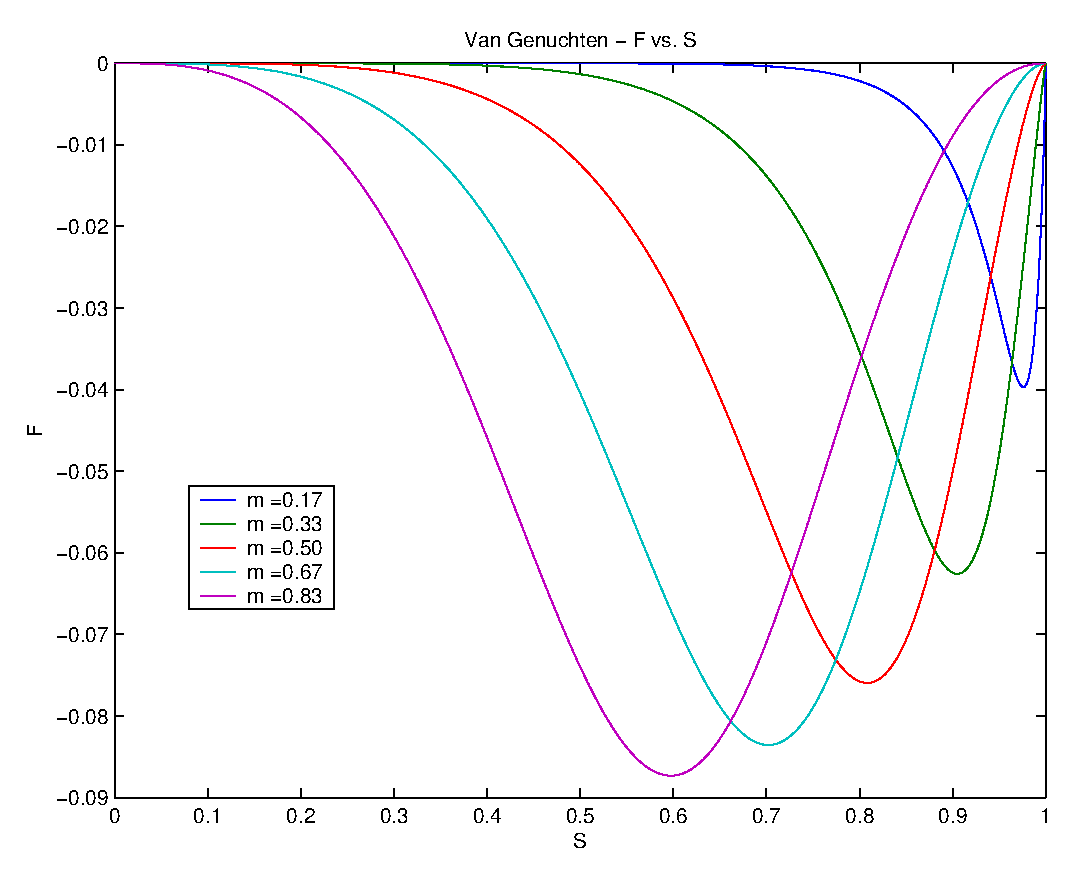
\epsfig{file=Fbl_S.eps,scale=0.4}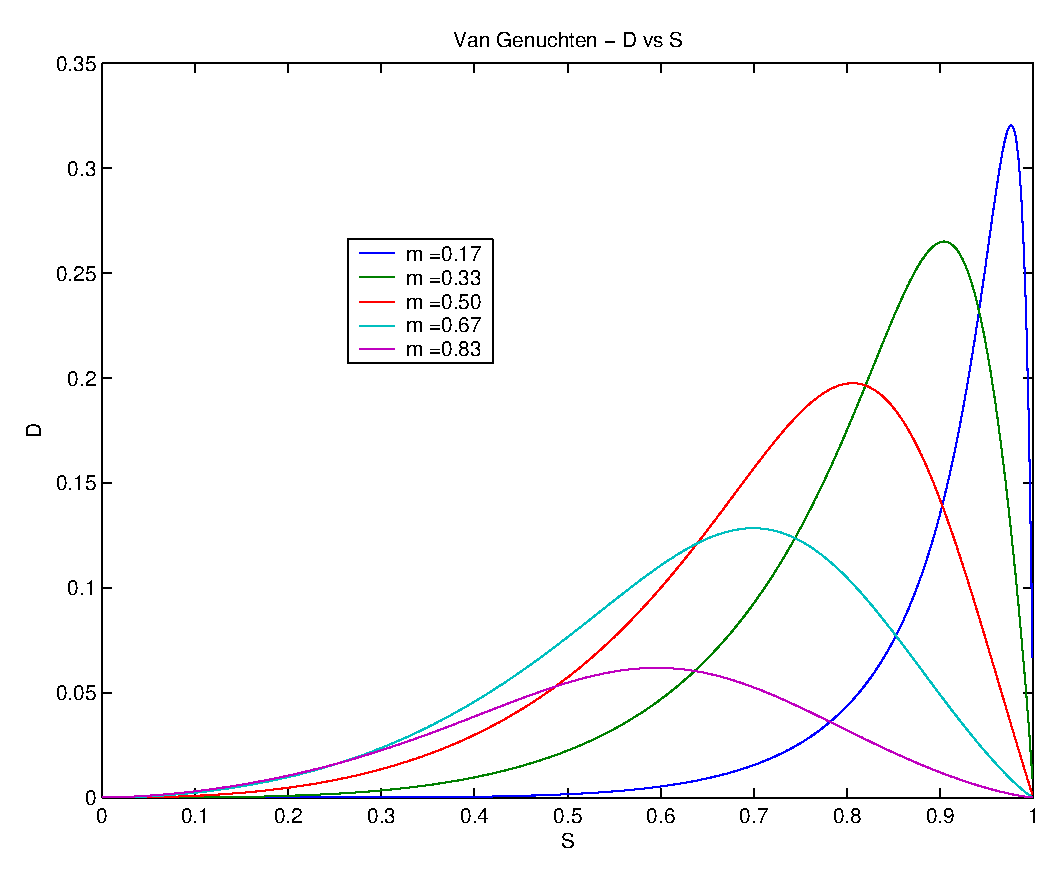
\epsfig{file=Dbl_S.eps,scale=0.4}
\caption{Buckley-Leverett: $F$ vs. $S$ (Left), $D$ vs. $S$ (Right) \label{blCoeff}}
\end{figure}
\begin{figure}
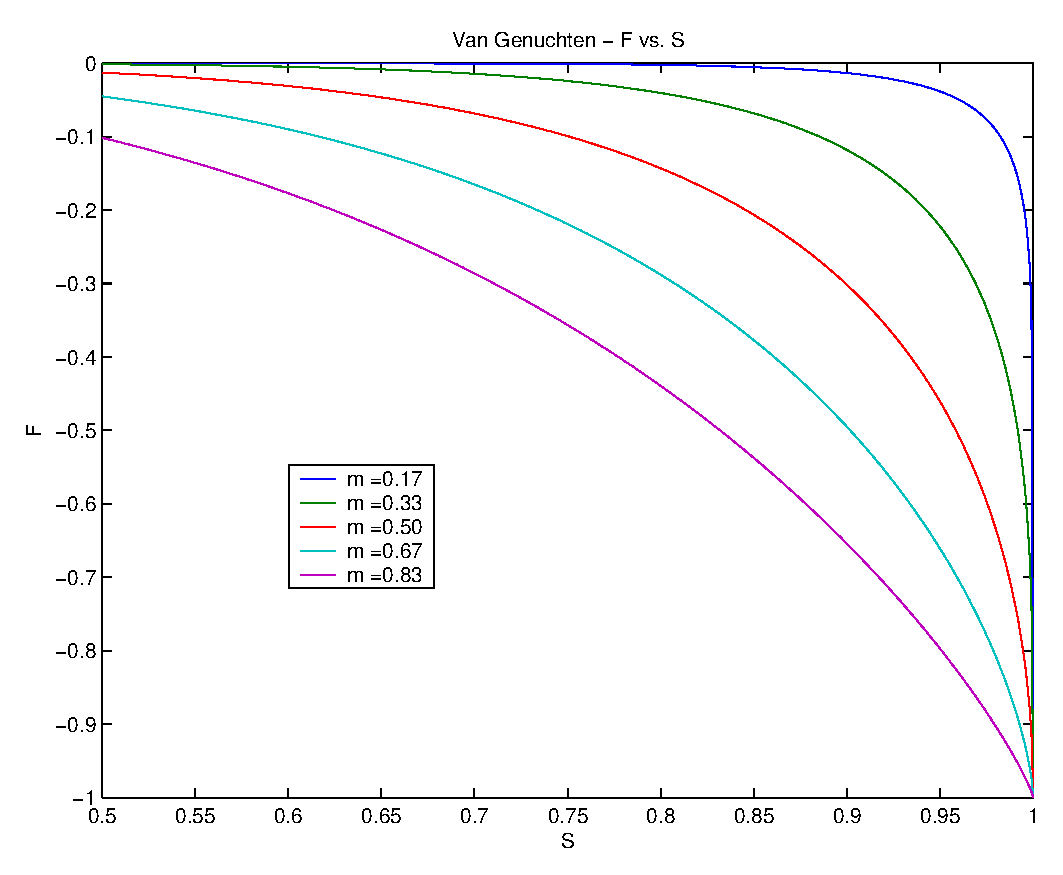
\epsfig{file=FvsS_VGM_RE.eps,scale=0.4}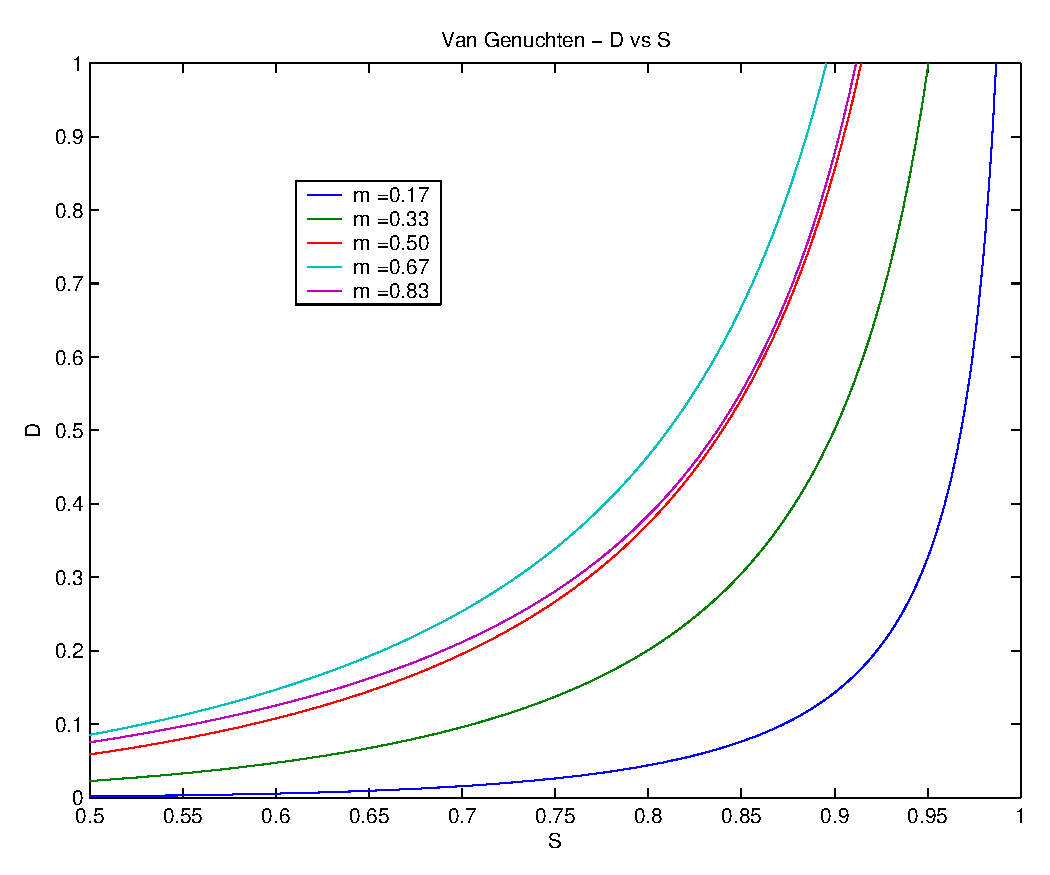
\epsfig{file=DvsS_VGM_RE.eps,scale=0.4}
\caption{Richards' Equation: $F$ vs. $S$ (Left), D vs. $S$ (Right) \label{reCoeff}}
\end{figure}
We will try to understand how these kinds of degeneracy affect the solutions. To focus on the behavior near $S=1$ we again use asymptotic approximations. For $u=1-S$ we have 
\begin{eqnarray}
\od{p_c}{S} &\sim& \frac{m-1}{m}\frac{1}{m}^{-m} u^{-m} \\
k_{rw} &\sim& 1-2 \frac{1}{m}^m u^m \\
k_{rn} &\sim& \frac{1}{m}^{2m} u^{\frac{1}{2}+2m}
\end{eqnarray}
Neglecting constants, for twophase flow we obtain
\begin{eqnarray}
  \label{eq:twopSimpCoef}
  D &\sim &  u^{\frac{1}{2}+m} \\
  F &\sim &  u^{\frac{1}{2}+2m} 
\end{eqnarray}
and for Richards' equation we have
\begin{eqnarray}
  D &\sim &  u^{-m} \\
  F &\sim &  u^m 
\end{eqnarray}
Since $(1-u^m)_x = (u^m)_x$ we will study the simplified model
\begin{equation}
  \label{eq:simpMod}
  u_t - \epsilon (u^p)_{xx} + g (u^q)_{x} = 0
\end{equation}
where $\epsilon > 0$ and $-\infty < g <\infty$ are constants. Note
that we've used the Kirchoff transformation on the diffusion
coefficient and also that \eqn{simpMod} is identical in form to
\eqn{reactTrans}. For reactive transport $p=q=1/r > 1$. For twophase
flow $p = 3/2 + m,q=1/2+2m$ so that $1<p<5/2$ and $0<q<5/2$. For
Richards' equation $p=1-m, q = m$ so $0<p,q<1$. We now try to
understand some qualitative aspects of \eqn{simpMod} for various
values of $p$ and $q$ occuring in the models above.

\msection{Finite Speed of Propagation} One property of 
solutions that is useful is the finite speed of propagation property,
which we define as follows (c.f. \cite{Gilding_Kersner_97}).  First consider
solutions of \eqn{simpMod} on the strip $(-\infty,\infty) \times
(0,T]$.  Next define the support of $u$ by $N(t) = \cbl x | u(x,t) > 0
\cbr$ and the front location $\zeta(t) = \sup \cbl x | u(x,t) > 0
\cbr$.  We say the solution has finite speed of propagation when
$\zeta(0) < \infty$ implies $\zeta(t) < \infty, 0 < t < \tau$ for some
$\tau \in [0,T]$. The finite speed of propagation property is
important for two reasons 1) the model will then predict that air
particles move into saturated regions at a finite speed and 2) the
solutions $u(x,t) = 1 - S(x,t)$ are generally non-Lipschitz continuous
in $x$ and $t$ at $\zeta(t)$.  According to \cite{King} \eqn{simpMod}
for initial conditions if and only if i) $p > 1$ and $q \geq 1$ or ii)
$q < 1$, $g>1$ and $p > q$.  Thus we will loose the finite speed of
propagation property for $g = -1$ and $m < 1/4$ for the simplified
twophase model and when $m < 1/2$ or $g=-1$ for the simplified
Richards' equation model.
  
\msection{Previous Work: Pressure Head Form} If $p$ or $q < 1$ then we
can transform \eqn{simpMod} to an equation with non-negative $C^1$
coefficients via $u=v^{1/r}$ for some $0<r<1$. For instance
$r=min(p,q)$ would work. This choice of variables would be nice
because the semi-discrete problem would have $C^1$ coefficients,
though it would have DAE dynamics rather than simple ODE dynamics.
Newton's method would converge quadratically if implicit time-stepping
were used. In the case of the pressure head form of Richards' equation
we're essentially taking $r=1/p$ which works if $m<1/2$ because $p<q$.
We trade non-Lipschitz behavior in the diffusion coefficient for a
degenerate time term. Note, however that the characteristic speeds are
unchanged by this transformation (they're still infinite) but that the
diffusion coefficient is uniformly elliptic (in fact it $D=1 at u=0$).
Thus degeneracy at $u=0$ can also be viewed as a change of type from
parabolic to elliptic.

For $m < 1/2$, however, the pressure head transformation no longer
works because $q<p$. Note however that simply switching to $v=^{1/q}$
yields
\begin{equation}
  \label{eq:simpMod}
  \frac{1}{q}v^{\frac{1}{q}-1} v_t - \epsilon (\frac{p}{q} v^{\frac{p}{q} - 1})_{xx} + g (v)_{x} = 0
\end{equation}
which has zero diffusion at $v=0$ ($p/q - 1 > 1$) while at the same
time characteristic speeds, being the same regardless of the choice of
variables, are infinite. The change of type corresponding to the
$m<1/2$ degeneracy is from parabolic to hyperbolic, but the roles of
time and space are reversed in the hyperbolic problem. 

There are two aspects of some of the previous work that I've glossed
over. First, the pressure head form is an extension of the saturation
form because it also provides additional information in the form of
the pressure distribution in the saturated zone. This involves the
additional assumption that the air pressure is atmospheric everywhere,
but I don't think that any significant numerical or theoretical
difficulties are caused by extending the range of the unknown. Second,
my work at least didn't focus on finding the right variable
transformation via asymptotics but rather by simply inverting the
non-Lipschitz coefficients. That is for a non-Lipschitz nonlinearity,
say $F(u)$, using the coefficient $F$ as a variable (i.e. if $F$ is
monotone by using the inverse as the variable transform either
directly or more generallay by adding a constraint with the zero level
set being the graph of $F(u)$ ) yields a formulation with smooth
coefficients. It may be that this approach has merit because in some
way it automates the process of finding the right variable transform
when the nonlinearities are very complex.

\msection{Barenblatt's Solution} We will now consider several special solutions in order to understand the solution dynamics. First we consider $g=0$, in which case the equation is the porous medium equation
\begin{equation}
  \label{eq:poMe}
  u_t - (u^p)_{xx} = 0
\end{equation}
By seeking a solution of the form $u(x,t) = t^{-\alpha}
v(xt^{-\beta})$ it can be shown that a solution for initial data is given by
(c.f.  \cite{Evans})
  \begin{equation}
    \label{eq:barenBlatt}
    u(x,t) = \frac{1}{t^{\frac{1}{p+1}}}\sbl b - \frac{p-1}{2p(p+1)} \pl \frac{x}{t^{\frac{1}{p+1}}} \pr^2 \sbr^{\frac{1}{p-1}} \quad |x| < \zeta(t)
  \end{equation}
  where $b$ is determined from the initial conditions corresponding to a point source $u(x,0) = M \delta(x,0)$. For $p > 1$ we have
  \begin{equation}
    \label{eq:front}
    \zeta(t) = \pl \frac{2p(p+1)}{p-1} b \pr^{1/2} t^{\frac{1}{p+1}}
  \end{equation}
  Thus the propagation speed is finite for $p>1$, for all $t$. Note
  also that $u_t$ and $u_x$ blow up at $\zeta(t)$ if $p > 2$. The case
  $p>2$ corresponds to two-phase flow with $m>1/2$ or reactive
  transport with $r< 1/2$. The case where $p<1$ corresponds to
  Richards' equation. Since in this case $p-1<0$ we have that
  $\zeta=\infty$ and the speed of propagation is infinite (the
  solution positive for all $x$ for $t>0$). Graphs of the solution are  given in \ref{bbSol}
\begin{figure}
\caption{Barenblatt's Solution \label{bbSol}}
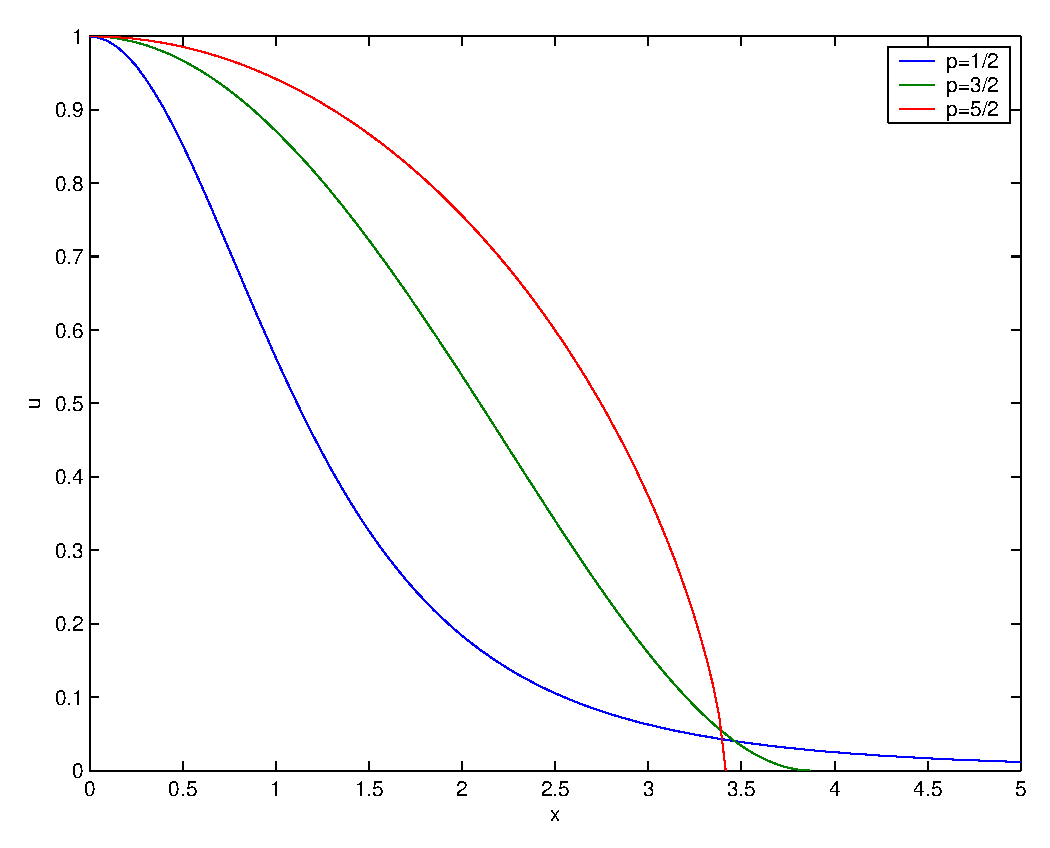
\epsfig{file=barenblatt.eps,scale=0.7}
\end{figure}

\msection{Boltzmann's Solution} We can also get a similary solution on
the half line by assuming $u(x,t) = u(xt^{-1})$. This solution is more
useful for numerical testing but more complicated to derive and
general only results in an integral equation rather than a closed form
solution. I'll add this later.

\msection{Taveling Wave Solutions} To find traveling wave solutions of
\eqn{kt} we assume that solution has the form $\phi(x,t) = \phi(x -
ct) = \phi(\eta)$ where $c$ is the wave speed. Assuming for now that
the traveling wave solution is bounded away from $S=0,1$ (the
non-differentiable points which are the same as the diffusion
degeneracies) \Eqn{kt} is then
\begin{equation}
  \label{eq:travWave}
  -c \od{S}{\eta} + \od{}{\eta}\sbl F - \od{\phi}{\eta} \sbr = 0
\end{equation}
Integrating once with respect to $\eta$ and rearranging yields
\begin{equation}
  \label{eq:travWavOde}
  \od{\phi}{\eta}  = -c S(\phi) + F(\phi) + b
\end{equation}
where $b$ is the constant of integration. We will enforce the following asymptotic boundary conditions on the \eqn{travWavOde}
\begin{eqnarray}
  \label{eq:odeBC}
  \lim_{\eta \rightarrow - \infty} \phi &=& \phi_{L} \\
\lim_{\eta \rightarrow \infty} \phi &=& \phi_{R} 
\end{eqnarray}
This implies the additional requirement
\begin{equation}
  \label{eq:lim}
  \lim_{\phi \rightarrow \phi_L,\phi_R} -c S(\phi) + F(\phi) + b = 0
\end{equation}
which in turn implies
\begin{equation}
  \label{eq:intConst}
  b = c S_L - F_L = c S_R - F_R
\end{equation}
where I've used the shorthand $S_L = S(\phi_L)$ etc. From \eqn{intConst} we can also determine $c$
\begin{equation}
  \label{eq:waveSpeed}
  c = \frac{F_R - F_L}{S_R - S_L}
\end{equation}
Note that \eqn{waveSpeed} is the Rankine-Hugoniot condition for the
hyperbolic model obtained by neglecting diffusion.  We will assume
$S_R > S_L$ and take $b=c S_L - F_L$. The traveling wave ODE is then
\begin{equation}
  \label{eq:odeFinal}
   \od{\phi}{\eta}  = F(\phi) - \sbl \frac{F_R - F_L}{S_R - S_L} (S(\phi) - S_L) + F_L\sbr = g(\phi_L,\phi_R,\phi)
\end{equation}
Solutions of the traveling wave equation exist and are unique when $g
> 0$ for $\phi_L < \phi < \phi_R$.This condition can be seen as
requiring the chord connecting $(S(\phi_L),F(\phi_L))$ and
$(S(\phi_R),F(S_R))$ to lie under the graph of $F(S(\phi))$. The
entropy condition for the hyperbolic model for a shock connecting
$S_L$ and $S_R$ is equivalent to $g>0$

This approach works fine for the non-degenerate case, but we've done
several things that require differentiability. C. J. van Duijn and P.
Knabner proved existence and uniqueness when $S(\phi)$ is
non-Lipschitz and $F$ is linear in $\phi$ (the reactive transport
model is an example of where this occurs). I'm working through their
paper to understand the approach. They define ``weak'' traveling waves
where only $c S(\phi) + \od{\phi}{\eta}$ is $C^1$. For our problem $F$
and possibly $S$ will be non-Lipschitz. For their case they give
detailed existence and uniqueness proofs.

\bibliographystyle{plainnat}
\bibliography{mp}
\end{document}